\documentclass[10pt]{report}
\usepackage[a4paper, top=2.5cm, left=2.5cm, bottom=2.5cm, right=2.5cm]{geometry}
\usepackage[english]{babel}
\usepackage{parskip}  % Try to replace paragraph indentations with white lines
\usepackage{xspace}   % Decides whether to put a space after a \newcommand
\usepackage[toc,page,title]{appendix}  % Use \begin{appendices} ... \end{} iso \appendix
\usepackage{amsmath,amssymb,bbm}
\usepackage{enumerate}  % Choose alternative numberings, e.g. \begin{enumerate}[a.]
\usepackage{listings}      % Code listings
\usepackage{pgf}           % Figures

\usepackage{color}
\definecolor{lightgrey}{rgb}{0.9,0.9,0.9}
\definecolor{darkgreen}{rgb}{0.0,0.6,0.0}

% Citations:
\usepackage[numbers]{natbib}  
\bibliographystyle{MvdS_number_url}  % Use [1], print url = field



\usepackage{fancybox}  % Use \ovalbox for key strokes

\newcommand{\ldf}{\usefont{OT1}{cmr}{m}{n}}     % Select default LaTeX font - Computer Modern Roman
%\newcommand{\ldf}{\usefont{OT1}{cmss}{m}{n}}     % Select default LaTeX font - Computer Modern Sans
%\newcommand{\ldf}{\usefont{OT1}{phv}{m}{n}}     % Select default LaTeX font - Helvetica
\newcommand{\ttbf}{\usefont{OT1}{lmtt}{bx}{n}}  % Select bold typewriter font

%\usepackage[font=sf]{caption}  % Use sans-serif font for float captions - not exactly Helvetica



\newcommand{\note}[1]{\color{red}\textbf{#1}\color{black}\xspace}
\newcommand{\marc}[1]{\color{red}\textbf{Marc: #1}\color{black}\xspace}

\newcommand{\myChapter}[1]{
  \chapter{#1}
  \minitoc  % Create a ToC of this chapter
}


% General expressions:
\newcommand{\eg}{\emph{e.g.}\xspace}
\newcommand{\ie}{\emph{i.e.}\xspace}
\newcommand{\etc}{\emph{et cetera}\xspace}
\newcommand{\ff}{\emph{ff}\xspace}

% CLI symbols:
\newcommand{\pipe}{$|$}      % Needed to avoid | in \index{}
\newcommand{\logor}{$|\,|$}  % Needed to avoid | in \index{}
\newcommand{\home}{\url{~}}  % Home directory


% Often used code names:
\newcommand{\NULL}{\code{NULL}}
\newcommand{\void}{\code{void}}
\newcommand{\stdout}{\code{stdout}}
\newcommand{\stderr}{\code{stderr}}

% Man pages:
\newcommand{\man}[2]{\texttt{man #1 #2}\xspace}
\newcommand{\mancmd}[1]{\texttt{man #1}\xspace}

% Code:
\newcommand{\prototype}[3]{\hspace*{2em}\texttt{#1} {\ttbf #2\ldf}(\texttt{#3});\xspace}  % function prototype
\newcommand{\var}[2]{\hspace*{2em}\texttt{#1} {\ttbf #2\ldf};\xspace}  % variable declaration
\newcommand{\code}[1]{\texttt{#1}\xspace}  % inline code
\newcommand{\codeb}[1]{\ttbf #1\ldf\xspace}  % inline bold code
\newcommand{\codeline}[1]{\hspace*{2em}\texttt{#1}}  % separate code line

\newcommand{\cli}[1]{\noindent\hspace*{2em}\code{\$ #1}}  % command line input
\newcommand{\clir}[1]{\noindent\hspace*{2em}\code{\# #1}}  % command line input root
\newcommand{\clo}[1]{\noindent\hspace*{2em}\code{#1}}  % command line output
\newcommand{\clitem}[1]{\item[\code{\$}] \code{#1}}  % cli in itemized list, with $ as bullet
\newcommand{\clitemb}[1]{\item[\codeb{\$}] \codeb{#1}}  % cli in itemized list, with $ as bullet - bold

\newcommand{\key}[1]{\Ovalbox{\texttt{#1}}\xspace}  % key press/combination
\newcommand{\keyb}[1]{\Ovalbox{\ttbf #1\ldf}\xspace}  % key press/combination bold


% Heat pumps
\newcommand{\COP}{\mathrm{COP}}  % COP in "math mode"
\newcommand{\COPh}{\COP_{\mathrm{heating}}}  % COP_heating in "math mode"

\newcommand{\Qh}{Q_{\mathrm{H}}}
\newcommand{\Qc}{Q_{\mathrm{C}}}
\newcommand{\Th}{T_{\mathrm{H}}}
\newcommand{\Tc}{T_{\mathrm{C}}}

\newcommand{\Tin}{T_{\mathrm{in}}}
\newcommand{\Tout}{T_{\mathrm{out}}}

\newcommand{\Ph}{P_{\mathrm{heat}}}
\newcommand{\Pheat}{P_{\mathrm{heat}}}
\newcommand{\Pc}{P_{\mathrm{cool}}}
\newcommand{\Pcool}{P_{\mathrm{cool}}}
\newcommand{\Pel}{P_{\mathrm{el}}}

\newcommand{\degr}{^\circ}
\newcommand{\tdeg}{$\degr$\xspace}
\newcommand{\degC}{\degr\mathrm{C}}
\newcommand{\tdegC}{$\degC$\xspace}

  % Custom commands

\usepackage[pdftex]{hyperref}
\hypersetup{
  colorlinks = true,  % They get a red box around them if false, better set colour to black?
  linkcolor = blue,
  filecolor=magenta,
  citecolor = blue,
  urlcolor = blue,
  % linkcolor = black,
  % citecolor = black,
  % urlcolor = black,
  pdftitle = House Model References,
  pdfauthor = Trung Nguyen,
  pdfsubject = House Models,
  pdfkeywords = house - models - Python,
  pdfcreator = TeXLive LaTeX2e on Gentoo Linux,
  pdfproducer = TN - TeXLive LaTeX2e on Gentoo Linux,
  bookmarksnumbered = true,  % Number sections in PDF toc
}

\usepackage[utf8]{inputenc}

\usepackage[onehalfspacing]{setspace}
\usepackage{float}
%\usepackage{biblatex}   % Using reference package
%\addbibresource{mybibliography.bib}

\usepackage[nottoc]{tocbibind} %Adds "References" to the table of contents
\usepackage{graphicx}






% Title page:
\title{House model}
\author{Trung Nguyen\\
HAN University of Applied Sciences\\
Arnhem, The Netherlands} %\\


\begin{document}
	
\ldf  % Set LaTeX default font

% Set up code listing style:
\lstset{
	language=Python,
	% Fonts:
	basicstyle=\ttfamily\footnotesize,
	%keywordstyle=\ttfamily,
	%identifierstyle=,
	%commentstyle=\ttfamily\scriptsize,
	% B/W code:
	% commentstyle=\ttfamily\itshape,  % Italic
	% stringstyle=\ttfamily,
	% identifierstyle=\ttbf,           % Bold typewriter type
	% keywordstyle=\ttbf,              % Bold tt
	% Colour:
	commentstyle=\scriptsize\ttfamily\color{brown},
	stringstyle=\ttfamily\color{darkgreen},
	identifierstyle=\color{blue},
	keywordstyle=\ttfamily\color{red},
	% Spaces:
	showstringspaces=false,
	breaklines=true,
	breakatwhitespace=true,
	% Line numbering:
	numbers=left,
	numberstyle=\tiny,
	stepnumber=2, 
	numbersep=5pt,
	% Frames:
	frame=single,
	frameround=tttt,
	backgroundcolor=\color{lightgrey},
	morekeywords={pthread_create},
}
%\renewcommand{\thelstlisting}{\thechapter.\arabic{lstlisting}}  % This is the default?
%\numberwithin{lstlisting}{section}  % AMSmath: number code listings per section
%\numberwithin{lstlisting}{chapter}  % AMSmath: number code listings per chapter


\maketitle

%\begin{center}
%	\today
%\end{center}

\tableofcontents

\newpage

% \chapter{Introduction}

\section{Introduction}

Building energy simulation is a vast field of research that started in the late 50’s and that is still highly active nowadays. Building energy simulations are mainly used to help taking design decisions, to analyze current designs and to forecast future building energy use. Building energy modelling methods can mainly be divided into three categories:
\begin{itemize}
  
    \item White box models (physics-based)
    \item Black box models (data-driven)
    \item Grey box models (hybrid)

\end{itemize}


White box models are based on the equations related to the fundamental laws of energy and mass balance and heat transfer. White box models can be differentiated in two types, \emph{distributed} parameter models and \emph{lumped} parameter models. Lumped parameter models simplify the description of distributed physical systems into discrete entities that approximate the behavior of a distributed system. The advantage of using lumped models is the decrease in simulation time \textbf{(Ramallo-González et al.\cite{Alfonso})}. White box models are of special interest for the design phase as they are used to predict and analyse the performance of the building envelope and building systems.
Black box models are based on the statistical relation between input and output system values. The statistical relation between input and output is based on actual data. The relation between the parameters can differ based on the amount of data and the method used to analyze the relation. Currently, there is a large and active field of research about statistical models that are used on black box models \textbf{(Coacley et al.\cite{Coakley})}. Black box models are of special interest when there is a large amount of actual input and output data available. 

Grey box models are hybrid models that aim to combine the advantages of both approaches. In order to use them it is necessary to implement some equations and it is also required to have actual data of inputs and outputs.

\newpage


\section{White box lumped model: RC network}
\subsection{White box lumped model}

The objective of the house model for this project is to serve as test environment for a heat pump model, what means that the house model is intended as a tool to help taking building systems design decisions. The house heating needs calculation model implemented for this project is a white box lumped model. Specifically, it is a RC network model consisting of resistances (R) and capacities (C). The RC network model is based on electrical systems analogy. The simulation of thermodynamic systems characterizing building elements as resistances or capacities allows to simplify the model while maintaining a high simulation results accuracy (Bagheri et al., Bacher et al.).  
There are several types of RC models, the most common being 3R4C models and 3R2C models which are applied on the outer and internal wall. For the simulation of simple house buildings 3R2C models perform as accurate as more complex 3R4C models (Fraisse et al. ). Considering that one of the objectives for this project is to obtain a fast but accurate simulation of a simple dwelling the 3R2C network model appeared as starting point. In the 3R2C model two indoor temperature nodes in the dwelling with capacities (usually an air and a wall temperature) and a well-known outdoor temperature are present. Between these 3 temperature nodes 3 heat transfer resistances are present. However, the direct heat transfer between the inner walls and the outdoor air is low. Moreover, uncertainties are present about heat transfer coefficients between walls and indoor air, different indoor temperatures in the house rooms and the ground temperature which deviates from the outdoor temperature. In addition, occupancy behaviour varies strongly. For that reason, we have made a further simplification to a 2R2C model. In section 4 it is shown that this dwelling model delivers a reliable annual energy consumption.


\subsection{House Model R and C Values}

This document presents the basic information for calculating a house model based on an RC network. This category of house models, analogous to electrical impedance networks, may have different numbers of R and C components, and may have various component topology. For the specific model properties, references will be given.

In heat transfer theory the basic thermal circuit contains thermal resistances. Heat transfer occurs via conduction, convection and radiation. In analogy with Ohm's Law for electricity, expressions can be derived for the heat transfer rate (analogous to electrical current) and the thermal resistances (analogous to ohmic resistances) in these three modes of heat transfer. The temperature difference plays a role analogous to the electrical voltage difference. These expressions are shown in Fig.\ref{table_1}.
\begin{figure}[H]
	\centering
	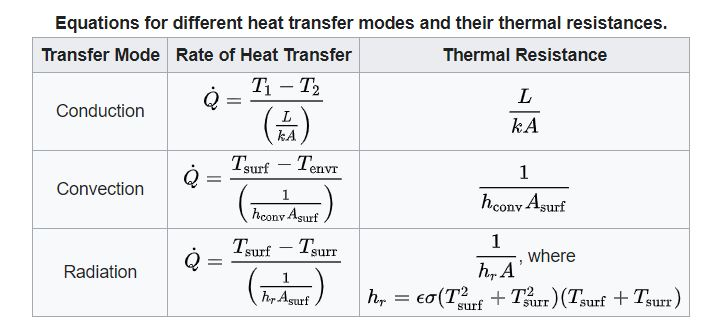
\includegraphics[width=0.8\columnwidth]{Pictures/heat transfer mode.JPG}
	\caption[Short title]{Heat transfer modes\cite{GIGO}}
	\label{table_1}
\end{figure}
\newpage
In \cite{HTTHERMO} and \cite{FUND} the expressions in Fig.\ref{table_1} are derived.
For conduction, the expression for $R_{th} = \frac{L}{k\dot A}$

$L$ is the distance over which heat transfer takes place, or the thickness of the material
$A$ is the conductive surface area

The units of $R_{th}$ are: $ [\frac{K}{W}] $

$ [W] = [\frac{W}{m \cdot K}] \dot [m^2] \cdot [\frac{K}{m}] $

The units of $k$ are: $ [\frac{m}{m^2} \cdot \frac{W}{K}] = [\frac{W}{m \cdot K}]$

Thermal conductivity of material $k = [\frac{W}{m \cdot K }] = [\frac{W}{m \cdot K }]  = [W \cdot m^{-1} \cdot K^{-1}]$

$k$ is also denoted as $\lambda$

Reference: \cite{ELECRESCOND}

Ohm's Law: $ R = \frac{U}{I} \quad [\frac{V}{A}] = [\Omega] $

Electrical resistivity: $ \rho = [\frac{\Omega \cdot m^2}{m} ] = [\Omega \cdot m] $ Material property.

Electrical conductivity: $ \sigma = \frac{1}{\rho} =[\frac{1}{\Omega \cdot m}] = [\frac{S}{m}] $ Material property.

Electrical resistance $ R = \frac{\rho \cdot L}{A} $ or $ R = \frac{L}{\sigma \cdot A} $
\\

Thermal Law: 
Heat flux $ \dot Q $ in $ [W \cdot m^{-2}] $

$ \dot Q = \frac{\Delta T}{R_{th}} \quad R_{th} = \frac{\Delta T}{\dot  Q} 
\quad [\frac{K}{W \cdot m^{-2}}] = [\frac{m^2 \cdot K}{W}]$

(Specific) Thermal resistivity: $ R_\lambda $ or $ r = [\frac{K}{W \cdot m^{-2}} \frac{1}{m} ] = [\frac{m \cdot K}{W}] $ Material property.

Thermal conductivity: $ \lambda $ or $ k  = \frac{1}{r} = [\frac{ W \cdot m^{-2} }{K} \cdot m] 
= [\frac{W}{m \cdot K}] $ Material property

Thermal resistance R-value or $ R_{th} = \frac{r \cdot L}{A} $ or $ R = \frac{L}{k \cdot A} $

Unit $ R_{th} = [\frac{m \cdot K}{W} \frac{m}{m^2}] = [\frac{m^2 \cdot K}{W}] $
\\

$R_c$-value $ = r \cdot L = \frac{L}{k} = \frac{L}{\lambda} $
\\

Some typical heat transfer thermal resistance values, also denoted as R\textsubscript{c}-values are: \cite{OVERALL}: 

\begin{itemize}
	\item Static layer of air, 40 mm thickness (1.57 in)  : R = 0.18 [$m^2K/W$].
	\item Inside heat transfer resistance, horizontal current : R = 0.13 [$m^2k/W$]. 
	\item Outside heat transfer resistance, horizontal current : R = 0.04 [$m^2K/W$].
	\item Inside heat transfer resistance, heat current from down upwards : R = 0.10 [$m^2K/W$].
	\item Outside heat transfer resistance, heat current from above downwards : R = 0.17 [$m^2K/W$].
	
\end{itemize}

\begin{figure}[H]
	\centering
	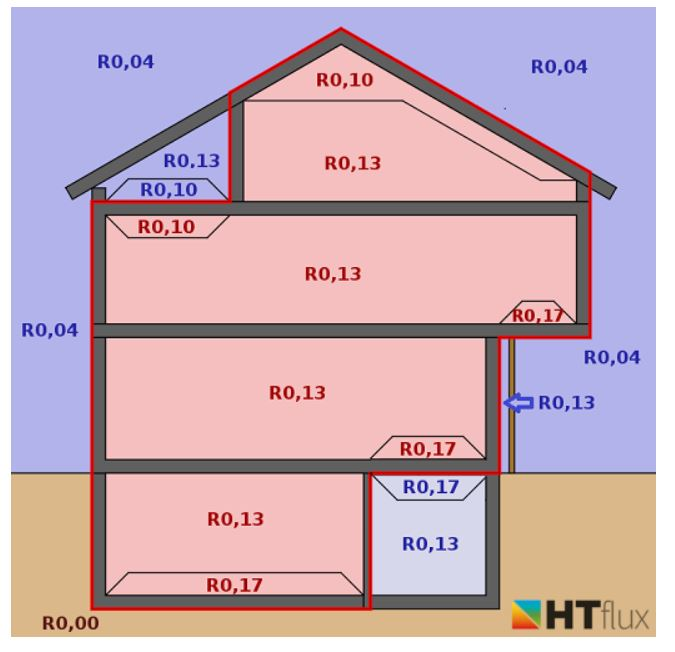
\includegraphics[width=0.8\columnwidth]{Pictures/Overview of heat resistances.JPG}
	\caption[Short title]{An overview of heat transfer resistance\cite{SURFREST}}
	\label{fig:overview}
\end{figure}


The standard R\textsubscript{c}-values that have been used for facades, roof and floor until 2020 are summarized in Fig.\ref{fig:Rcvalues}:

\begin{figure}[H]
	\centering
	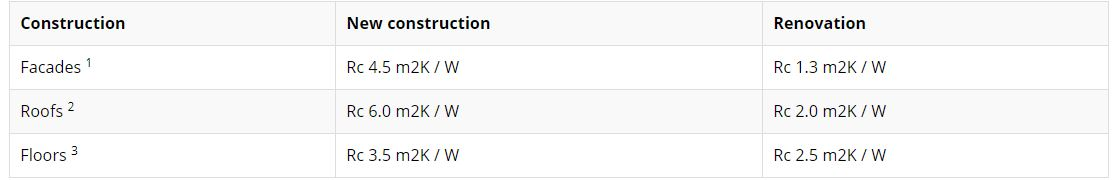
\includegraphics[width=1.0\columnwidth]{Pictures/Rc_values_2020.JPG}
	\caption[Short title]{Rc Values \cite{ISOL}}
	\label{fig:Rcvalues}
\end{figure}

New standard values will be used from 1-1-2021, since the building standard NEN 1068 will be replaced by the NTA 8800 standard. The old and new situation is described in "EnergieVademecum Energiebewust ontwerpen van nieuwbouwwoningen", chapter 5: Thermische isolatie, thermische bruggen en luchtdichtheid.
\cite{ISSO}.

\begin{figure}[H]
	\centering
	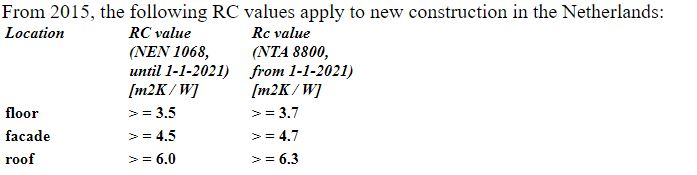
\includegraphics[width=1.0\columnwidth]{Pictures/Rc_values_2021.JPG}
	\caption[Short title]{Rc Values \cite{RVALUE}}
	\label{fig:newRc}
\end{figure}

The values used for different types of houses such as: row houses, detached houses and apartments can be found in the document "Voorbeeldwoningen 2011" \cite{VOORBEELD}. An example with values for a common type of row house, built in the period from 1975 to 1991 is shown in Fig.\ref{row_house}:


\begin{figure}[H]
	\centering
	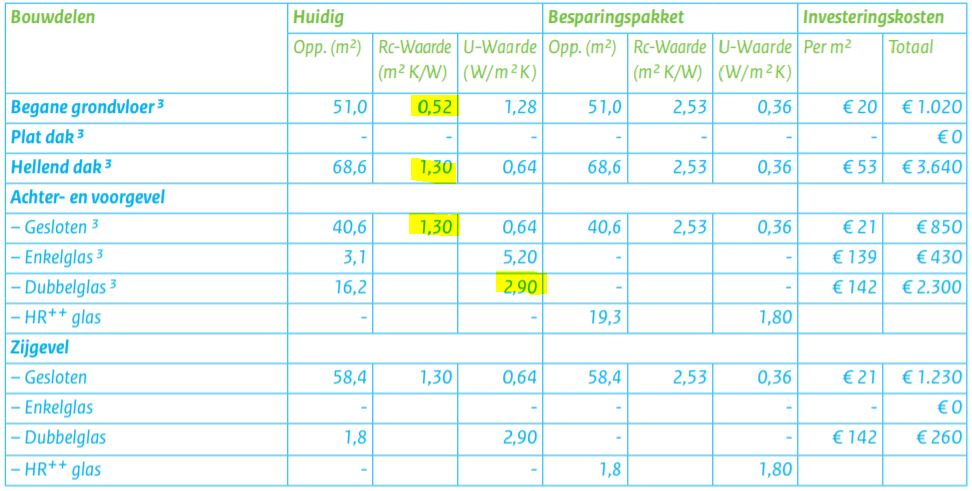
\includegraphics[width=0.8\columnwidth]{Pictures/row_house_1975-1991.JPG}
	\caption[Short title]{R\textsubscript{c}-values for a row house type built between 1975-1991 \href{Voorbeeldwoningen 2011 bestaande bouw.pdf}{[7].}}
	\label{row_house}
\end{figure} 


\newpage


\section{Simulink model user guideline}

The dwelling model has been fist developed in Matlab/Simulink and convert to Python later on. In the Simulink model it is possible to define the dwelling characteristics, the dwelling use data and the climate data. With some of this information the model resistances and capacities are built on a Matlab script. The resistances and capacities values are used during the year energy simulation. 
In sections 2.1 to 2.3 the information provided to make the simulation is presented. In section 2.4 it is explained how the 2R2C network model has been build.

\subsection{Dwelling characteristics information}
	
The dwelling characteristics taken into account in order to define the model resistances and capacities are presented in figure 2.1. The ventilation rate n in ach (air changes per hour) is based on a mechanical ventilation rate of 150 m3/h for kitchen, toilet and bathroom) by regulations.

\begin{figure}[H]
	\centering
	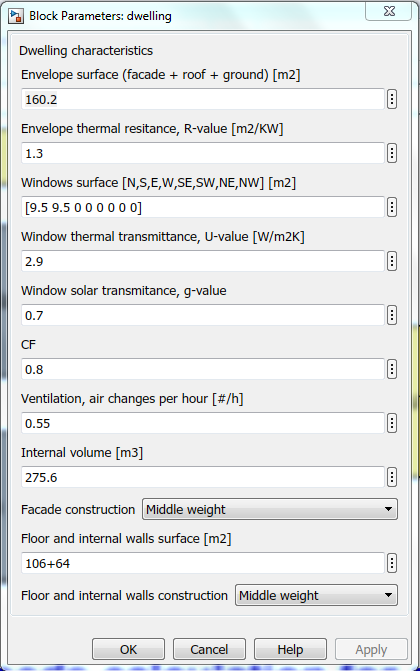
\includegraphics[width=0.8\columnwidth]{Pictures/dwelling characteristic model information.png}
	\caption[Short title]{Dwelling characteristic model information}
	\label{figure: Dwelling characteristic}
\end{figure}
\newpage
\subsection{Dwelling use data}

The dwelling use data define the schedule to be used to calculate the dwelling internal heat and the thermostat set-points. The thermostat signal is communicated to the heat pump model. The information use to define the dwelling use is presented in Figure 2.2
\\
\begin{figure}[H]
	\centering
	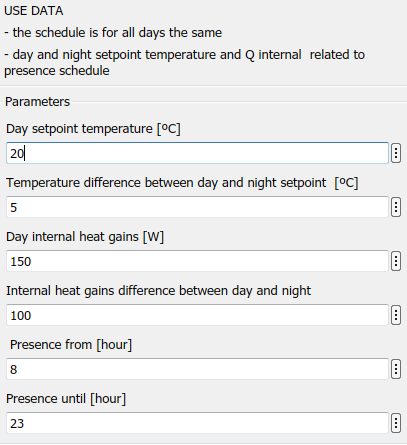
\includegraphics[width=0.8\columnwidth]{Pictures/Dwelling use model information.png}
	\caption[Short title]{Dwelling use model information}
	\label{figure:Dwelling info}
\end{figure}
\newpage
\subsection{Climate data}

The hourly data about the outdoor temperature and the solar radiation is extracted from the NEN5060:2018 norm. This norm defines a typical meteorological year using the Finkelstein-Schafer statistical method with the climate data of 20 years period (1996-2015). The meteorological data used by the norm is updated once every 5 years.  

The typical meteorological year data is the one to be used when calculating the typical energy use of the heating installation. The NEN norm offers also three other hourly climate data sets, each one with a different perceptual deviation from the typical meteorological year: 1\%, 3\% and 5\%. These data sets are to be used when analysing the response of the heating installation under more extreme climate conditions. This is usually done for design installation purposes. The total energy use calculated with these other data sets will not give a reliable value for calculating the typical energy use.  In figure 2.3 it is shown that is it possible to choose between the four different NEN climate data sets. 

\begin{figure}[H]
	\centering
	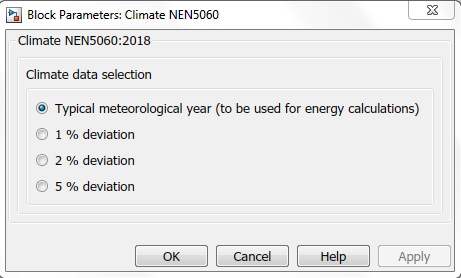
\includegraphics[width=0.8\columnwidth]{Pictures/climate data selection.png}
	\caption[Short title]{Climate data selection}
	\label{figure Climate data selection}
\end{figure}

In a pre-process the global incident radiant is calculated for North, South, East, West, North-West, North-East, South-West and South-East orientations of the façade in Matlab. The model from Perez is applied for the exchange. In this model the irradiation is split into a direct and diffuse terms.
\newpage


\section{Dwelling (envelope) model analogous to a 2R-2C network}

The 2R-2C house model structure is implemented as described below:
	
\begin{figure}[H]
	\centering
	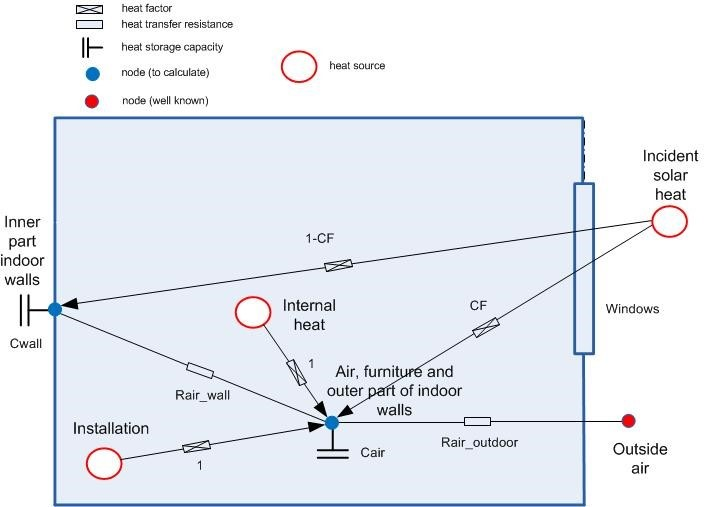
\includegraphics[width=1.0\columnwidth]{Pictures/envelopRC.jpg}
	\caption[Short title]{Schematic of envelope model}
	\label{fig:envelope2R2C}
	\end{figure} 
	
The equivalent electrical 2R-2C network with components and topology is given in Fig. \ref{fig:elec2R2C}.

\begin{figure}[H]
	\centering
	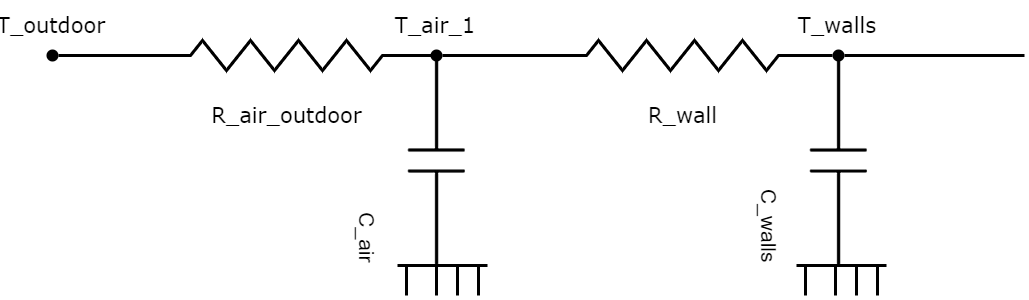
\includegraphics[width=1.0\columnwidth]{Pictures/2R2C_Model.png}
	\caption[Short title]{2R-2C house model}
	\label{fig:elec2R2C}
	\end{figure}
	
The model consists of two capacitances C\textsubscript{air, indoor} and C\textsubscript{wall} and two resistances R\textsubscript{wall} and R\textsubscript{air, outdoor}. The incident solar energy is divided between C\textsubscript{wall} and C\textsubscript{air} through the convection factor CF. It is assumed that both internal heat (lighting, occupancy and electric devices) and supplied heat (installation) initially heat up the indoor air. In Fig. \ref{fig:elec2R2C}, they are fully released at the T\textsubscript{air} node. 

 It is also assumed that furniture and the surface part of the walls have the same temperature as the air and the wall mass is divided between the air and wall mass. Thus, the capacity of the air node consists of the air capacity, furniture capacity and capacity of a part of the walls. \textbf{Appendix A} presents the coefficients in the dwelling model. In the resistance R\textsubscript{air, outdoor} the influence of heat transmission through the outdoor walls and natural ventilation is considered. 
 
For the air and wall nodes the following energy balances can be set up: 

\begin{equation}
C_{air}\frac{dT_{air}}{dt}=\frac{T_{outdoor}-T_{air}}{R_{air_{\_}outdoor}} + \frac{T_{wall}-T_{air}}{R_{air_{\_}wall}} + \dot{Q}_{inst} + \dot{Q}_{internal} + CF\cdot\dot{Q}_{solar}
\end{equation}

\begin{equation}
C_{wall}\frac{dT_{wall}}{dt}=\frac{T_{air}-T_{wall}}{R_{air_{\_}wall}} + (1-CF)\cdot\dot{Q}_{solar}
\end{equation}

 \begin{itemize}
      \item CF: Convection factor (solar radiation): the convection factor is the part of the solar radiation that enters the room and is released directly convectively into the room
      \item $\dot{Q}_{inst}$: delivered heat from heating system (radiator) [W].
      \item $\dot{Q}_{solar}$: heat from solar irradiation [W].
      \item $T_{air}$: indoor air temperature $^o$C.
      \item $T_{outdoor}$: outdoor temperature $^o$C.
      \item $T_{wall}$: wall temperature $^o$C.
      \item $R_{air_{\_}wall}$: walls surface resistance [$\frac{K}{W}$].
      \item $R_{air_{\_}outdoor}$: outdoor surface resistance [$\frac{K}{W}$].
      \item $C_{air}$: air capacity [$\frac{J}{K}$].
      \item $C_{wall}$: wall capacity [$\frac{J}{K}$].
    \end{itemize}
    

Total heat transfer of solar irradiation through the glass windows. 
\begin{equation}
Q_{solar}=g.\sum(A_{glass}.q_{solar})
\end{equation}

\begin{itemize}
    \item $q_{solar}$: solar radiation on the outdoor walls [$\frac{W}{m^2}$]. 
    \item g: g value of the glass (ZTA in dutch) [0..1]\cite{zontoetreding}
    \item A: glass surface [$m^2$].
\end{itemize}

%7.6.6.1.2 Ramen met niet-verstrooiende beglazing NTA8800
%https://help.dgmr.nl/bink9/zontoetredingsfactor-zta.html
%https://www.joostdevree.nl/shtmls/zta.shtml
%ISSO-Handboek Zonnestraling: 5.5.1 en 5.2

\newpage

\section{Simulation, results and verification}

\subsection{Simulation}
In order to calculate the inside temperature of the house the model considers five heat flow. 

\begin{itemize}
    \item Transmission
    \item Ventilation
    \item Solar Gains
    \item Internal Heat Gains
    \item Heating/Cooling
\end{itemize}

The model also considers the mass of the air inside the house and the mass of the walls.  
House characteristics data.

The document Voorbeeldwoningen 2011 Bestaande bouw published by Agentschap NL \cite{VOORBEELD} will be used as a reference to determine the house characteristics. The document makes a classification of the house stock per construction type (7) and year of construction (4 time periods).  

\textbf{Construction type.}
\begin{itemize}
    \item Detached house (vrijstaande woning)
    \item Semi-detached house (2 onder 1 kap woning)
    \item Terraced house (rijwoning)
    \item Apartment block own access (maisonnettewoning)
    \item Apartment horizontal shared access (galerijwoning)
    \item Apartment block vertical shared access (portiekwoning)
    \item Apartment block in general (flatwoningen (overig))
    
\end{itemize}
\textbf{Year of construction.}
\begin{itemize}
    \item Build before 1964
    \item Build between 1965 and 1974
    \item Build between 1975 and 1991
    \item 	Build between 1992 and 2005
\end{itemize}

For the first model, the data of a detached house building build between 1975 and 1991 has been used. 
The energy consumption sum presented in the report as the first validation mechanism for this model. In the following model development, we should look for the possibility to validate the model with the use of real data.

\textbf{Climate data.}\\
NEN 5060:2008 and 2018 nl (Hygrothermische eigenschappen van gebouwen -Referentieklimaatgegevens), will be used as the climate data for the simulations.

\textbf{Internal heat gains data.}\\
There is no reference document about the internal heat gains for dwelling in the Netherlands. We can consider that there are two people living in the house with an average working schedule.
Control mechanism
The heating will be controlled by a thermostat. The indoor temperature of the house is based on recommendation given on the ISSO publication Kleintje Binnenklimaat. The indoor temperature should be maintained at a minimum of 20 degrees. 
We could consider taking cooling into account. 


\subsection{Results}
To test the model, we have used the data from the document Voorbeeldwoningen 2011 Bestaande bouw published by Agentschap NL \cite{VOORBEELD}. We have run the model for a detached house building build between 1975 and 1991 and for row house building build between 1975 and 1991.For the detached house the model calculates a sum of the yearly energy needs of 10545 kWh. The document Voorbeeldwoningen 2011 gives a calculated energy use for heating and hot water of 1542 m3 gas. The average gas consumption of hot tap water on a Dutch household is 300 m3gas. We assume a combustion (under) value ho=35.2 MJ/m3 gas. Taking into consideration a heating system efficiency of 0.9, the energy need is 10843 kWh. 


\begin{equation}
\frac{(1542-300) \cdot 35200}{3600\cdot 0.9}= 10843[KWh] 
\end{equation}


For the row house the model calculates a sum of the yearly energy needs of 19776 kWh. The sidewalls have been considered as adiabatic walls. The document Voorbeeldwoningen 2011 gives a calculated energy use for heating and hot water of 2616 m3 gas. The average gas consumption of hot tap water on a Dutch household is 300 m3gas. Taking into consideration a heating system efficiency of 0.9, the energy need is 20219 kWh. 

\begin{equation}
\frac{(2616-300) \cdot 35200}{3600\cdot 0.9}= 20129[KWh] 
\end{equation}

The results give an indication that the model is on the right result range for detached and row house.

The plot on figure \ref{fig:Simulationresults}, show the comparison of simulation results and annual heating consumption in Voorbeeldwoningen 2011 \cite{VOORBEELD}. More results can be found in Appendix B

\begin{figure}[H]
	\centering
	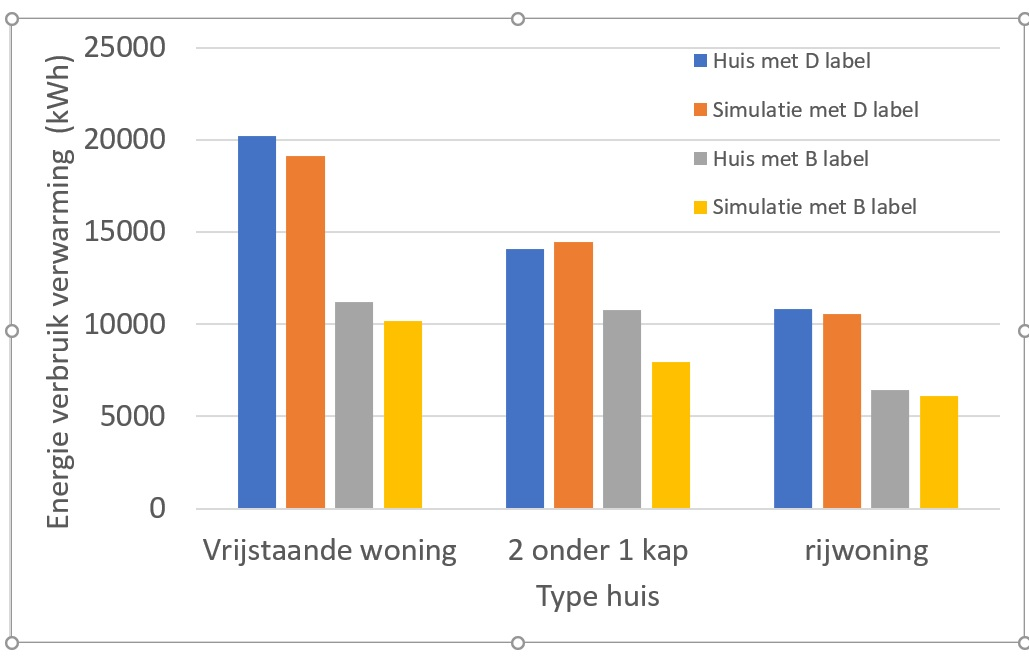
\includegraphics[width=1.0\columnwidth]{Pictures/Simulation results.jpg}
	\caption[Short title]{Simulation versus energy usage}
	\label{fig:Simulationresults}
	\end{figure}
\newpage

The graph in figure \ref{fig:heatingvstemp} shows the yearly heating demand needed for difference outdoor temperature.
It is clearly show the typical whether condition in the Netherlands where most of the energy use for heating happen at temperature range from 4 to 8 degree $^oC$.

\begin{figure}[H]
	\centering
	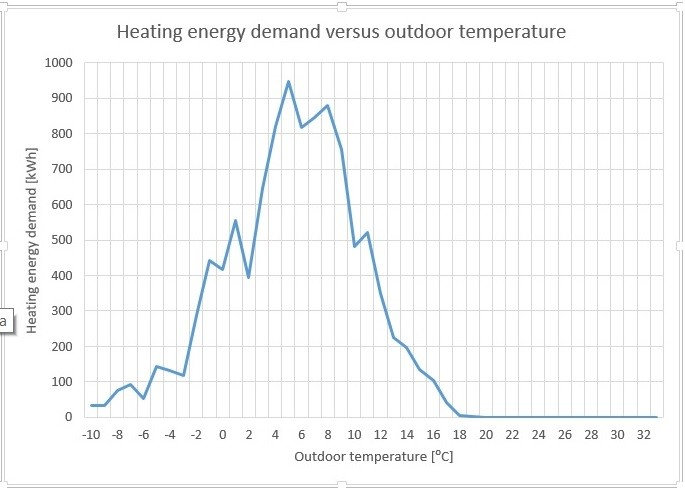
\includegraphics[width=1.0\columnwidth]{Pictures/Yearheatingdemand.jpg}
	\caption[Short title]{Simulation versus energy usage}
	\label{fig:heatingvstemp}
	\end{figure}
	
In order to get an estimation of the minimum heating power capacity needed to maintain a specific indoor temperature for the whole year the model thermostat has been set at a constant temperature day and night.
Minimum heating power capacity needed to maintain a specific indoor temperature has been shown in table 1.

\begin{table}[H]
    \centering
    \begin{tabular}{|c|c|}
    \hline
    Indoor temperature $[^oC]$  & Minimum heating powercapacity $[W]$ \\
    
    \hline
     18     &  6041 \\
     
     \hline
     19     &  6335 \\
     
     \hline
     20     &  6474 \\
     
     \hline
     21     &  6704 \\
     
     \hline
     22     &  6972 \\
     
     \hline
     23     &  7144 \\
     
     \hline
     24     &  7366 \\
     
    \hline

    \end{tabular}
    \caption{Minimum heating powercapacity}
    \label{tab:Minimumheat}
\end{table}
 
\newpage


\section{2 Zones house model 7R-4C network}

The 7R4C structure implemented is shown in Figure \ref{fig:schematic7R4C}.
	
\begin{figure}[H]
	\centering
	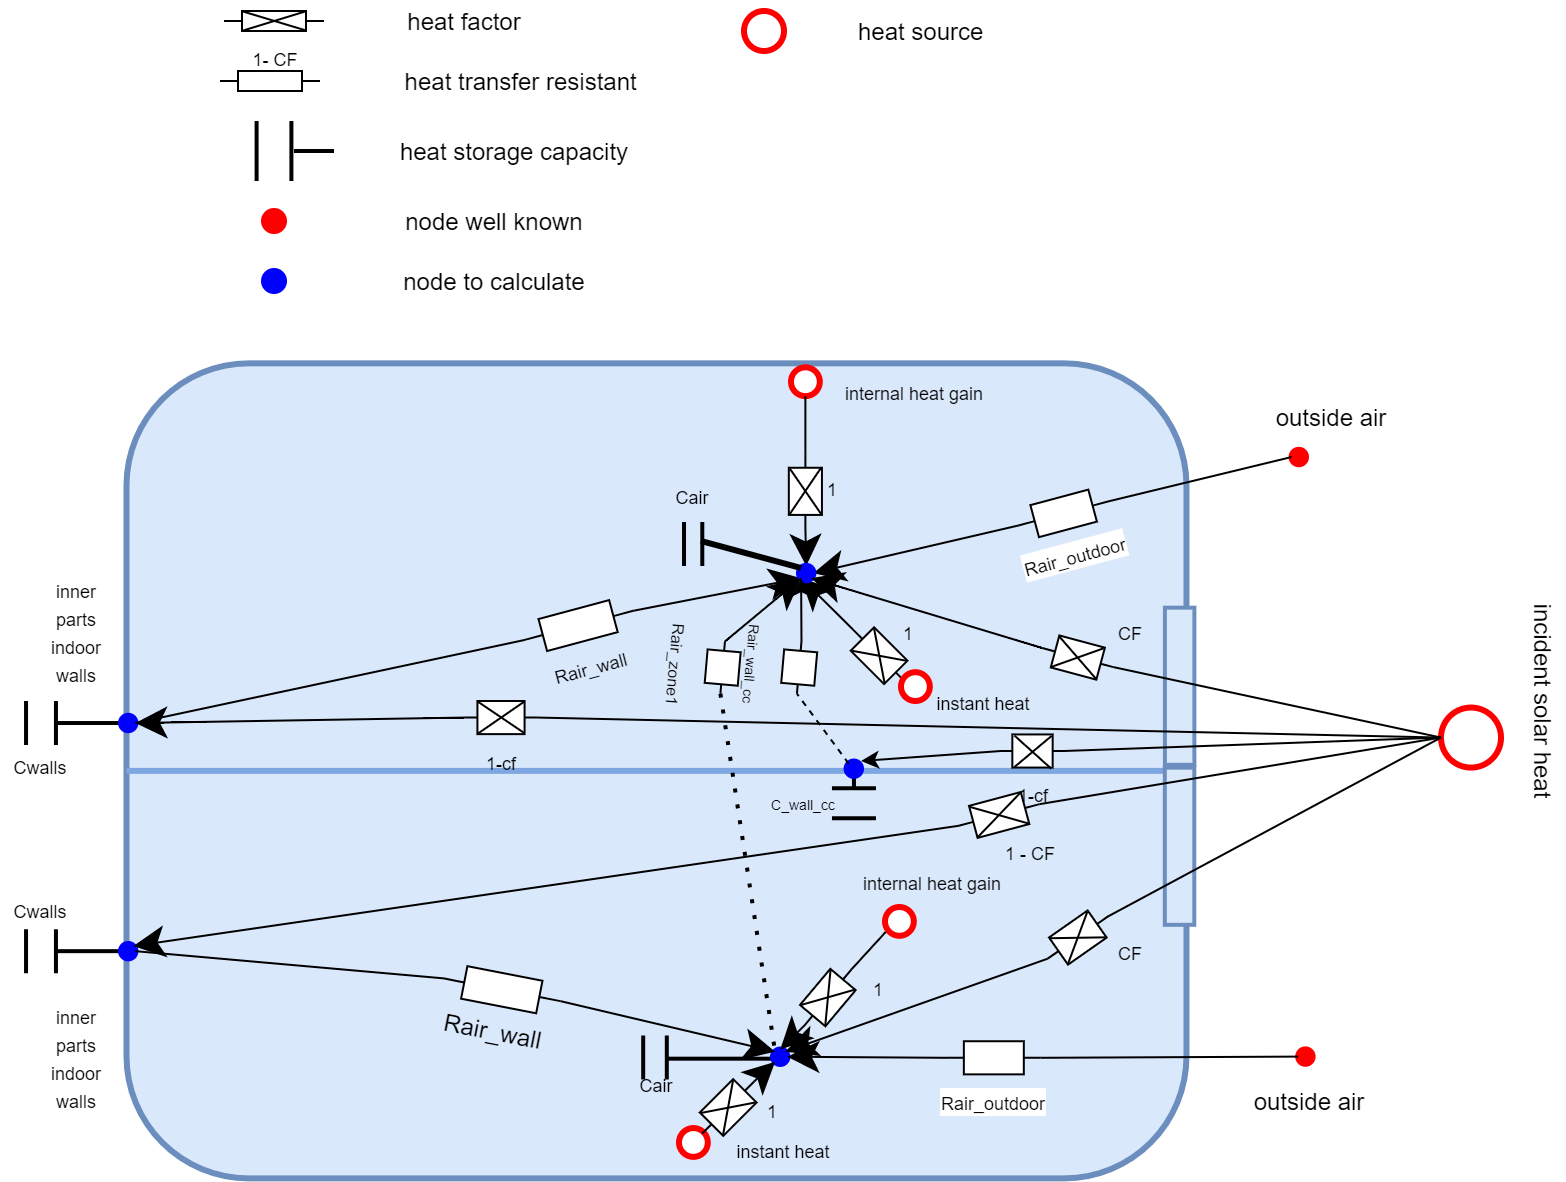
\includegraphics[width=1.0\columnwidth]{Pictures/House_electrical_circuits overview.png}
	\caption[Short title]{Schematic of 2 zones house model}
	\label{fig:schematic7R4C}
	\end{figure} 
	
The equivalent electrical 7R-4C network with components and topology is given in Fig. \ref{fig:eq7R4C}.

\begin{figure}[H]
	\centering
	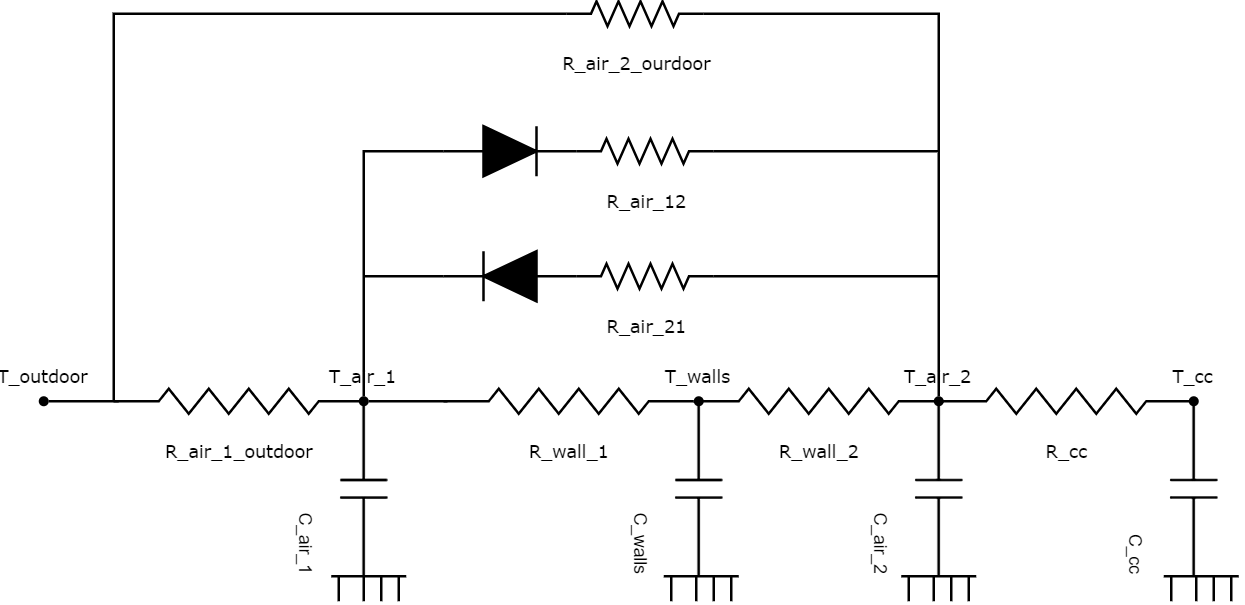
\includegraphics[width=1.0\columnwidth]{Pictures/2_Zones_house_circuits.png}
	\caption[Short title]{R-C circuits of 2 zones house model}
	\label{fig:eq7R4C}
	\end{figure}

with:\\
\begin{itemize}
    \item \texttt{T\_outdoor} : outdoor temperature [$\degr C$] 
    \item \texttt{T\_air\_1}  : zone 1 air temperature [$\degr C$]
    \item \texttt{T\_walls}   : wall temperature [$\degr C$]
    \item \texttt{T\_air\_2}  : zone 2 air temperature [$\degr C$]
    \item \texttt{T\_cc}      : temperature of the concrete layer between zone 1 and zone 2 [$\degr C$]
    \item \texttt{R\_air\_1\_outdoor} : outdoor resistance valus.
    \item \texttt{R\_wall\_1} : walls resistance value.
    \item \texttt{R\_wall\_2} : walls resistance value.
    \item \texttt{R\_cc}      : concrete resistance value.
    \item \texttt{R\_air\_12} : resistance value of air flow from zone 1 to zone 2.
    \item \texttt{R\_air\_21} : resistance value of air flow from zone 2 to zone 1.

\end{itemize}

\newpage

\chapter{NEN and ISO}

The list of NEN and ISO standard used in the calculation:

\begin{itemize}
    \item NTA 8800
    \item NEN 1068
    \item ISO 6946
    \item ISO 10077-2
    \item NEN 7120
\end{itemize}

%\newpage

\appendixname{A}
\appendix
\section{Dwelling parameters calculation}
The initial parameters value for House model (row house 1975 to 1991) are listed in the table below\cite{VOORBEELD}:
    
\begin{tabular}{|p{3cm}||p{7cm}||p{3cm}||p{3cm}|}
 \hline
 \multicolumn{4}{|c|}{Initial Parameters Value} \\
 \hline
\textbf{Abbreviation} & \textbf{Description} & \textbf{Value} & \textbf{Units}\\
 \hline
 
$A_{facade}$ & Envelope surface (facade + roof + ground)   & 160.2 &  $m^2$\\
 \hline

$A_{internal{\_}mass}$ & Floor and internal walls surface    & 170 & $m^2$\\
 \hline

 $V_{dwelling}$ & Internal volume & 275.6 &$m^3$\\
  \hline

 $Rc_{facade}$ & Envelope thermal resistance, R-value & 1.3 &  $\frac{m^2}{kw}$\\
  \hline

 $U_{glass}$& Window thermal transmittance, U-value & 2.9 &$\frac{W}{m^2k}$\\
 \hline

n & Ventilation, air changes per hour  & 0.55 & $[number/h]$\\

\hline

 CF& Convection factor & 0.8 &\\
 \hline
 
 $N_{facade}$ &Facade construction & Light weight = 0/ Middle weight = 1/ Heavy weight = 2 &  \\
 \hline
 
  $th_{facade}$& Construction thickness: Light weight / Middle weight / Heavy weight  & [ 0.1,  0.1, 0.2 ] & m \\
 \hline
  
 $c_{facade}$& Specific heat capacity construction [J/kgK] & [840, 840, 840] &$\frac{J}{KgK}$\\
 \hline
 
 $\rho_{facade}$& Density construction: Light weight / Middle weight / Heavy weight  & [500, 1000, 2500] &$\frac{kg}{m3}$\\
 \hline
 

 $N_{internal{\_}mass}$& Floor and internal walls construction & Light weight = 0/ Middle weight = 1/ Heavy weight = 2 &\\
 \hline
 
 $th_{internal{\_}mass}$& Construction thickness: Light weight / Middle weight / Heavy weight & [ 0.1,  0.1, 0.2 ] & m \\
 \hline
 
 $c_{internal{\_}mass}$& Specific heat capacity construction & [840, 840, 840] &$\frac{J}{KgK}$\\
 \hline
 
 $\rho_{internal{\_}mass}$& Density construction: Light weight / Middle weight / Heavy weight  & [500, 1000, 2500] &$\frac{kg}{m3}$\\
 \hline
 
 $\rho_{air}$& Density air & 1.20 &$\frac{kg}{m3}$\\
 \hline
  
 $c_{air}$& specific heat capacity air  & 1005 &$\frac{J}{KgK}$\\
 \hline
 
 $\alpha_{i{\_}facade}$ & Interior surface thermal resistance $R_{i} =\frac{1}{\alpha_{i{\_}facade}}$  (Rc-Waarde=0.13,ISO 6946) & 8 & \\
 \hline
 
 $\alpha_{e{\_}facade}$ & Exterior surface thermal resistance $R_{se} =\frac{1}{\alpha_{e{\_}facade}}$ (0,04 $\frac{m^2k}{W}$ ,ISO 6946,external surfaces or external side of exterior wall) & 23 &$\frac{W}{m^2k}$\\
 \hline
 
 $\alpha_{internal{\_}mass}$& Interal wall thermal resistance $ R_{air{\_}wall} = \frac{1}{A_{internal{\_}mass} \cdot \alpha_{internal{\_}mass}} $ Resistance indoor air-wall  & 8 &$\frac{W}{m^2k}$\\
 \hline
 
 $\rho_{internal{\_}masss}$& Density construction in [kg/m3] & 1 &$\frac{W}{m^2k}$\\
 \hline

\end{tabular}
\\

Volume floor and internal walls construction [m3]: $V_{internal,mass} = A_{internal,mass} \cdot th_{internal,mass}$

Ventilation, volume air flow [m3/s] : $qV = \frac{n \cdot V_{dwelling}}{3600} $  

Ventilation, mass air flow [kg/s] : $qm = qV \cdot \rho_{air} $  
\newline

Calculation of the resistances.
\newline

Resistance indoor air-wall: $R_{air_{\_}wall} = \frac{1}{A_{internal,mass} \cdot \alpha_{internal,mass}} $ 

U-value indoor air-facade: $U =\frac{1}{\frac{1}{\alpha_{i{\_}facade}}   + R{c{\_}facade} + \frac{1}{\alpha_{e{\_}facade}}}$ 

Resistance indoor air-outdoor air: $R_{air{\_}outdoor} = \frac{1}{A_{facade} \cdot U + A_{glass} \cdot U_{glass} + qm \cdot c_{air}}$ 
\newline

Calculation of the capacities.
\newline

Capacity indoor air and walls: $C_{air} =\frac{rho_{internal{\_}mass} \cdot c_{internal{\_}mass} \cdot V_{internal{\_}mass}}{2} + \rho_{air} \cdot c_{air} \cdot V_{dwelling}  $ 

Capacity walls : $C_{wall} =\frac{rho_{internal{\_}mass} \cdot c_{internal{\_}mass} \cdot V_{internal{\_}mass}}{2}$   

\newpage
  

\appendixname{B}
\section{R and C Values explanation.}

In \cite{HTTHERMO} and \cite{FUND} the expressions in Fig.\ref{table_1} are derived.
For conduction, the expression for $R_{th} = \frac{L}{k\dot A}$


The units of $R_{th}$ are: $ [\frac{K}{W}] $

$ [W] = [\frac{W}{m \cdot K}] \dot [m^2] \cdot [\frac{K}{m}] $

The units of $k$ are: $ [\frac{m}{m^2} \cdot \frac{W}{K}] = [\frac{W}{m \cdot K}]$

Thermal conductivity of material $k = [\frac{W}{m \cdot K }] = [\frac{W}{m \cdot K }]  = [W \cdot m^{-1} \cdot K^{-1}]$

$k$ is also denoted as $\lambda$

Reference: \cite{ELECRESCOND}

Ohm's Law: $ R = \frac{U}{I} \quad [\frac{V}{A}] = [\Omega] $

Electrical resistivity: $ \rho = [\frac{\Omega \cdot m^2}{m} ] = [\Omega \cdot m] $ Material property.

Electrical conductivity: $ \sigma = \frac{1}{\rho} =[\frac{1}{\Omega \cdot m}] = [\frac{S}{m}] $ Material property.

Electrical resistance $ R = \frac{\rho \cdot L}{A} $ or $ R = \frac{L}{\sigma \cdot A} $
\\

Thermal Law: 
Heat flux $ \dot Q $ in $ [W \cdot m^{-2}] $

$ \dot Q = \frac{\Delta T}{R_{th}} \quad R_{th} = \frac{\Delta T}{\dot  Q} 
\quad [\frac{K}{W \cdot m^{-2}}] = [\frac{m^2 \cdot K}{W}]$

(Specific) Thermal resistivity: $ R_\lambda $ or $ r = [\frac{K}{W \cdot m^{-2}} \frac{1}{m} ] = [\frac{m \cdot K}{W}] $ Material property.

Thermal conductivity: $ \lambda $ or $ k  = \frac{1}{r} = [\frac{ W \cdot m^{-2} }{K} \cdot m] 
= [\frac{W}{m \cdot K}] $ Material property

Thermal resistance R-value or $ R_{th} = \frac{r \cdot L}{A} $ or $ R = \frac{L}{k \cdot A} $

Unit $ R_{th} = [\frac{m \cdot K}{W} \frac{m}{m^2}] = [\frac{m^2 \cdot K}{W}] $
\\

$R_c$-value $ = r \cdot L = \frac{L}{k} = \frac{L}{\lambda} $

\newpage


%\bibliography{mybibliography}
\printbibliography[heading=bibintoc]


% \bibliography{mybibliography}

\end{document}



